\documentclass[12pt]{scrreprt}
\usepackage{graphicx}
\usepackage{geometry}
\geometry{
 a4paper,
 left=20mm,
 right=20mm,
 top=25mm,
 headheight=20mm,
 headsep=0mm,
 bottom=30mm,
}
\usepackage[T1]{fontenc}				% Trennung von Umlauten.
\usepackage[ngerman]{babel}	
\usepackage[utf8]{inputenc}
\usepackage[headsepline]{scrlayer-scrpage}
\ModifyLayer[addvoffset=-10pt]{scrheadings.head.below.line}
\usepackage{blindtext}
\usepackage[font=small,labelformat=empty,justification=centering]{caption}
\setlength{\parindent}{0em}

%Autordaten
\newcommand{\datum}{18.06.2020}
\newcommand{\autorinfo}{\textbf{Wechler, Tim-Jonas} (1137877)}


\ihead{\textbf{WT 1} \datum}
\chead{\autorinfo}
\ohead{\vspace{10pt}
\includegraphics[width=4cm]{logo_simple}}
 
\begin{document}
In der Vorlesung des 18.06.2020 ging es um die Umformung von metallischen Stoffen, der Zugversuch mit dem Spannungs- Dehnungs-Diagramm und zum Schluss die Gefüge mit der dazugehörigen Analyse.\par\vspace{5pt}
Bei der Umformung metallsichen Stoffe gibt es zwei Arten, diese sind Warmumformung und Kaltumformung. 
Die \textbf{Warmumformung} findet oberhalb der Rekristallisationstemperatur und ermöglicht so mit eine leichte Formgebung des Werkstücks. Durch kneten des Werkstoffs werden die mechanische Eigenschaften verbessert und die Korngröße geht über in ein kleiner, feinere Struktur.
Die \textbf{Kaltumformung} liegt hingegen unterhalb der Rekristallisationstemperatur, die verformung erhöht die Härte des Werkstoffs senkt aber die Bruchdehnung.\par\vspace{5pt}
Mit dem \textbf{Zugversuch} werden die mechanische Kenngrößen eines Werkstoffs ermittelt. Durch diesen Versuch kann man bei einer bestimmten Kraft gewisse Reaktionen des Werkstoffs erkennen.
Diese Reaktionen sind reversible Verformung, irreversible Verformung und Bruch.
Bei der \textbf{reversiblen Verformung} kommt der Werstoff nach gewisser Zeit oder soft wieder in seinen Ursprungsform zurück. 
Hat der Werkstoff hingegen eine \textbf{irreversible Verformung} vor so bleibt der Werkstoff in dieser Form, er geht nicht in seine Ursprungsform zurück.
Zu letzt kommt der \textbf{Bruch}, hier reist der Werkstoff da er eine überbelastung erfährt und das Material reist. In der Abbildung kann man eines Spannungs- Dehnungs-Diagramm sehen und die Zustände/Reaktionen eines Werkstoffs während des Zugversuchs.\par\vspace*{10pt}
\vspace*{-5mm}
\begin{figure}[h]
	% minipage mit (Blind-)Text
    \begin{minipage}{0.4\textwidth} 
        In dem roten Bereich ist die Probe noch elastisch und geht in seine Ursprungsform zurück.
        Im Lüdersbreich findet eine Umstrukturierung der Fremdatome statt, er ist auch optisch zusehen, es bilden sich im 45° Winkel Streifen aus. 
        Der nächste Bereich (Gleichmaßdehnungsbereich) ist der Bereich in dem sich der Werkstoffs sich weiter streckt aber nicht in seine ursprüngliche From zurückkehrt.
        Der Einschnürbereich ist dadruch markant das die Spannung im Werkstoff nach lässt und das Material stark an einer Stelle auseinander zieht.
        Zum Schluss kommt der Bruch. An dieser Stelle endet die Kennlinie. 
	\end{minipage}
	% Auffüllen des Zwischenraums
	\hfill
	% minipage mit Grafik
	\begin{minipage}{0.55\textwidth}
	% \textwidth bezieht sich nun auf die Minipage
	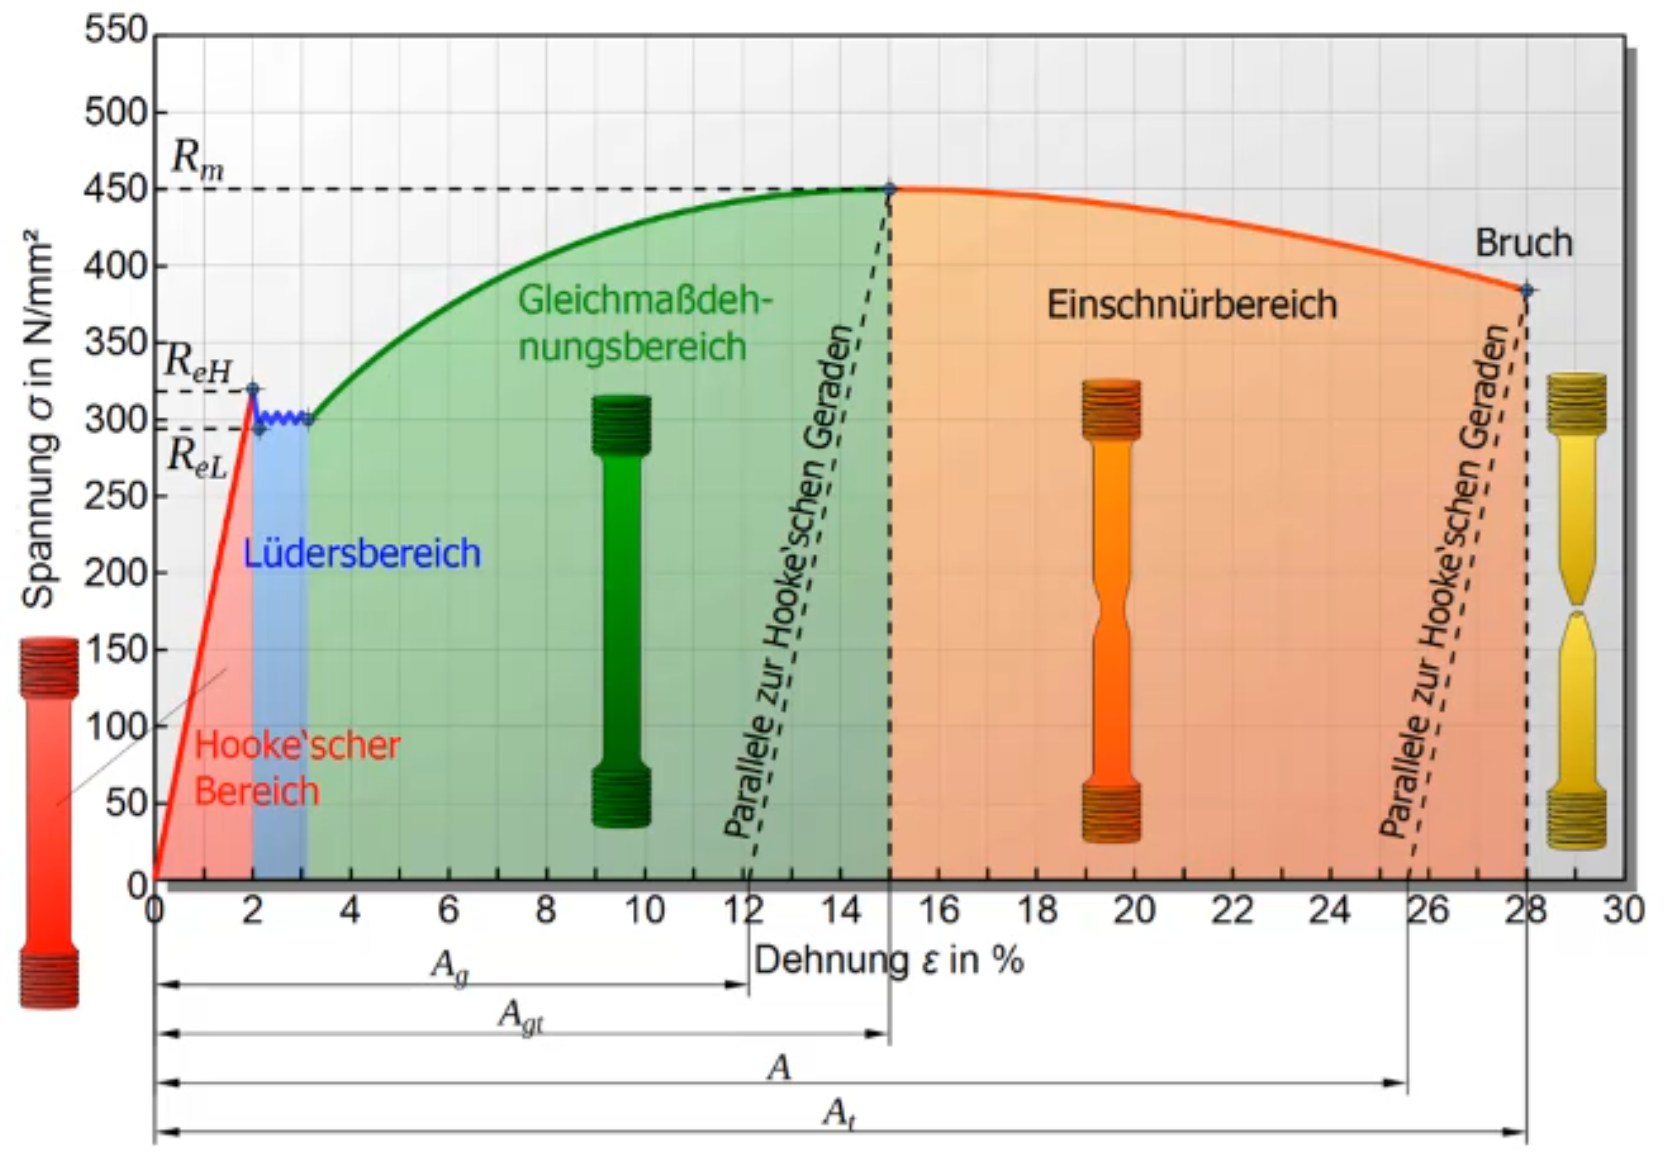
\includegraphics[width=\textwidth]{spannungsdiagramm.png}
	\caption{Spannungs- Dehnungs- Diagramm \\(Quelle: Vorlesungsfolien WT1 Dr.\,E.Geberth)}
	\end{minipage}
% \caption{noch eine Caption}
\end{figure}

Als nächstes komme ich zum Gefüge von Werkstoffe. Man unterscheidet vier Arten von Gefüge. Das \textbf{Primärgefüge} entsteht beim abkühlen der Schmelze. Als nächstes das \textbf{Sekundärgefüge}, aus dieser Art besteht der Werkstoff nach dem verformen oder einer Wärmebehandlung. Das \textbf{Mikrogefüge} ist nur unter dem Mikroskop sichtbar wohingegend das \textbf{Makrogefüge} mit bloßem Auge sichtbat oder unter einer einfachen Lupe.
Im Anschluss wurde uns über der Herstellung einer Schlifffläche näheres erklärt. Diesen Prozess kannte ich schon, da ich bei der Firma Memminger-IRO GmbH in Dornstetten in der Qualitätssicherung von Werkstoffen die Härte bestimmen sollte. 
Um dies durch zuführen benötigt man auch eine sehr glatte Oberfläche, leider kann ich mich an die Eckdaten nicht mehr erinnern.  
Nachdem die Fläche eine ausreichende Beschaffenheit für die untersuchung hat wird sie noch nachbehandelt damit man die eine Gefügeanalyse durchführen kann.\par
\vspace{5pt}
Die Gefügeanalyse kann auf drei Arten Daten erfassen, die wie folgt heißen, Flächenanalyse, Linearanalyse und Punktanalyse. Bei der Analyse wird von einem 2-dimensionalen Verhältnis auf das 3-dimensionale Verteilung einer gewählten Phase in der Probe zurückgeschlossen.
Die \textbf{Flächenanalyse} berechnet das Verhältnis zwischen der Phasenfläche und der gewählten Testfläche. 
Mit der \textbf{Linearanalyse} werden belieben Linien nacheinander auf der Testfläche gelegt, sie enden immer an einer Korngrenze. Bei einer einzelnen Linie wird dann ermittelt wie viele Körner einer Phase diese schneiden und welche Länge die Körner auf der Linie haben. Alle Messwerte der gleichen Phase werder ins Verhältnis zu der Gesamtlänger aller Linien gezogen. 
Bei der \textbf{Punktanalyse} wird über die Testfläche ein Raster gelegt anhand dessen Punkte gelegt werden. Im Anschluss wird dann gezählt wie viele Körner einer Phase auf diesen gewählten Punkten liegen. Die Anzahl der gezählten Punkte wird mit der Gesamtpunktzahl ins Verhältnis gesetzt.\par
\vspace{5pt}
Abschließend als Fazit kann ich sagen das es vieles neues gab, was sich auf die Gefügeanalyse bezieht und vereinzelnde Details in Spannungs- Dehnungs-Diagramm. Genauso war aber auch manches sehr bekannt für mich, was sich vorallem die Herstellung der Testfläche für die Gefügeanalyse bezieht. 
Hinzufügen muss ich auch, dass ich jetzt nach dem sechsten Lerntagebuch seine Art des Lernes wirklich komplett verstanden habe. 
Diese Art des Lernen schätze ich mehr als das reine Lernen auf eine Klausur, da man sich auf ein ganz andere Weise mit dem Stoff auseinandersetzt. Ich werde sehr wahrscheinlich dieses Prinzip auf weitere Fächer anwenden.

\end{document}

